\chapter{Lecture 9 - LU Factorization}
\label{ch:lec9n}
\section{Objectives}
The objectives of this lecture are to:
\begin{itemize}
\item Quantify the computational work of Gauss elimination.
\item Describe the LU factorization.
\item Demonstrate how to use the LU factorization for solving systems of equations.
\end{itemize}
\setcounter{lstannotation}{0}

\section{Computational Work of Gauss Elimination}

Throughout this course we have taken a rather crass approach to the amount of work done by the computer.  This reflects, in part, a basic reality that for many undergraduate students of engineering, most of the computer-based work comprises time that students spend writing and debugging code.  The amount of time that the computer actually spends executing the program, in many cases, is trivial.  

Looking ahead to some of the numerical methods that will be learned in this course, the situation will change.  Programs that analyze initial boundary value problems based on the finite difference method or finite element method will need to solve large systems of linear or non-linear equations.  These systems of equations are often large---it is not unusual to have millions of equations and unknowns---and the time that the computer spends assembling and solving these equations becomes significant.  Applications of this type are so important that modern high performance computing systems are regularly benchmarked based on how fast they can solve such problems.\cite{HPL,top500}     

In this section will will undertake a high-level analysis of the computational work required to perform Gauss elimination.  We will break this analysis into two parts: a) the forward elimination phase; and b) the back-substitution phase.

\subsection{Forward Elimination}
MATLAB code for the forward elimination phase is shown in the listing below:
\begin{lstlisting}[style=myMatlab]
for j = 1:n-1 /*!\annotation{lst:ann9n-1}!*/
    for i = (j+1):n /*!\annotation{lst:ann9n-2}!*/
        m = A(i,j)/A(j,j); % calculate pivot /*!\annotation{lst:ann9n-3}!*/
        A(i,j:n) = A(i,j:n) - m*A(j,j:n); /*!\annotation{lst:ann9n-4}!*/
        
        b(i) = b(i) - m*b(j); % update the right hand side /*!\annotation{lst:ann9n-5}!*/
    end
end
\end{lstlisting}

\vspace{0.1cm}

\noindent \ref{lst:ann9n-1} The outer loop, \lstinline[style=myMatlab]{for j=1:n-1...end}, will be traversed $\mathcal{O}(n)$ times.\sidenote{Here we adopt \emph{``Big oh''} notation.  It is used to charactarize the complexity and running time of an algorithm in asymptotic fashion.  So in this case, $\mathcal{O}(n)$ means that, as $n\to\infty$, the running time of this part of the code increases linearly with $n$.  Small details like constant factors are ignored.  It also means that lower order terms get ignored.  For example, a function that requires $n^3 + n^2 + n$ calculations would be characterized as $\mathcal{O}(n^3)$ since, as $n\to\infty$, the $n^2$ and $n$ terms become insignificant relative to $n^3$.}

\vspace{0.25cm} 

\noindent \ref{lst:ann9n-2} The inner loop, \lstinline[style=myMatlab]{for i=(j+1):n...end}, also will be traversed $\mathcal{O}(n)$ times.  

\vspace{0.25cm}

\noindent \ref{lst:ann9n-3} This line performs one floating point operation (FLOP) to calculate the pivot.

\vspace{0.25cm}

\noindent \ref{lst:ann9n-4} This line performs $\mathcal{O}(n)$ floating point operations.  These include multiplication of a vector by a scalar and vector addition.

\vspace{0.25cm}

\noindent \ref{lst:ann9n-5} This line performs two FLOPs: scalar multiplication and scalar addition.

\vspace{0.25cm}

\noindent Overall the forward-elimination part of the algorithm requires: $\mathcal{O}(n) \times \mathcal{O}(n) \times \mathcal{O}(n)$ operations to traverse the two nested loops and carry out the operations inside. The asymptotic operation count is thus: $\mathcal{O}(n^3)$.

\subsection{Back-Substitution}
MATLAB code for the back-substitution phase is shown in the listing below:
\begin{lstlisting}[style=myMatlab]
x = nan(n,1); 
for i = n:-1:1    /*!\annotation{lst:ann9n-6}!*/
   x(i) = (b(i) - ...    /*!\annotation{lst:ann9n-7}!*/
       A(i,(i+1):n)*x((i+1):n))/A(i,i);    
end
\end{lstlisting}

\vspace{0.25cm}

\noindent \ref{lst:ann9n-6} This loop is traversed $\mathcal{O}(n)$ times.

\vspace{0.25cm}

\noindent \ref{lst:ann9n-7} This line performs $\mathcal{O}(n)$ FLOPS for vector dot product, scalar addition and division.

\vspace{0.25cm} 

\noindent Overall, the back-substitution part of the algorithm requires: $\mathcal{O}(n) \times \mathcal{O}(n)$ operations; the asymptotic operation count is therefore: $\mathcal{O}(n^2)$.

\vspace{4.25cm}

\newthought{Taken together}, the entire Gauss elimination algorithm requires $\mathcal{O}(n^3) + \mathcal{O}(n^2)$ operations for a total asymptotic complexity of: $\mathcal{O}(n^3)$.  For large enough matrices, if you double the matrix size, the computer will need to perform a factor of $\approx 2^3$ more floating point operations and, roughly speaking, can be expected to take $2^{3}$ times as long. This is shown in Figure \ref{fig:lec9n-compute-vs-n}.
\begin{marginfigure}
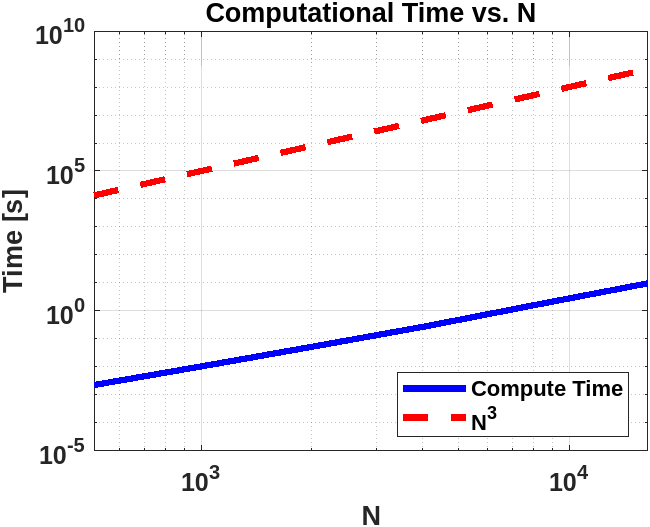
\includegraphics{lec9n_compute_vs_n.png}
\caption{Computing time vs. $n$ for Gauss elimination.}
\label{fig:lec9n-compute-vs-n}
\end{marginfigure}

\setcounter{lstannotation}{0} % do a re-set of the counter
\section{LU Factorization}
One problem with the Gauss elimination algorithm as described so far is this:  if you want to repeat the solution with a different right-hand-side, you would need to repeat all of the work you had just done.  We will not cover it in this class, but one possible solution to this problem is to devise an algorithm like Gauss elimination\sidenote{The Gauss-Jordan elimination does this.} that, in addition to solving the problem for the unknown vector $x$, also finds $A^{-1}$, the inverse of $A$.  With the inverse, we could find $x$ for a new right hand side with a simple matrix-vector multiplication.
\begin{align*}
Ax &= b \\
A^{-1}Ax &= A^{-1}b \\
Ix &= A^{-1}b \\
\Rightarrow x &= A^{-1}b
\end{align*}
As asymptotic analysis will readily show, matrix multiplication has $\mathcal{O}(n^2)$ complexity, so we can re-compute $x$ for any new $b$ in a small fraction of the time that it would take to re-perform Gauss elimination.  
We will not do this, however.  Instead we will perform a \emph{factorization} of $A$ in such a way that we can solve the linear system, $Ax=b$, with $\mathcal{O}(n^2)$ operations, for any new right hand side, $b$. This is called the \emph{LU factorization} and it is both faster and more-accurate (in floating point arithmetic) than finding the matrix inverse.\cite{higham-matrix-inverse} 

The LU factorization decomposes an invertible matrix into:
\begin{itemize}
\item A lower triangular matrix L; and
\item an upper triangular matrix U
\end{itemize}
such that $A = LU$.  It turns out that, while carrying out the Gauss elimination algorithm we actually computed the elements of the LU factorization:
\begin{equation*}
\underbrace{
\bracketMatrixstack{
a_{11} & a_{12} & a_{13} & a_{14} \\
a_{21} & a_{22} & a_{23} & a_{24} \\
a_{31} & a_{32} & a_{33} & a_{34} \\
a_{41} & a_{42} & a_{43} & a_{44}
}
}_{
A
}
=
\underbrace{ 
\bracketMatrixstack{
1 & 0 & 0 & 0 \\
m_{21} & 1 & 0 & 0 \\
m_{31} & m_{32} & 1 & 0 \\
m_{41} & m_{42} & m_{43} & 1
}
}_{
L
}
\underbrace{
\bracketMatrixstack{
a_{11} & a_{12} & a_{13} & a_{14} \\
0 & a^{\prime}_{22} & a^{\prime}_{23} & a^{\prime}_{24} \\
0 & 0 & a^{\prime \prime}_{33} & a^{\prime \prime}_{34} \\
0 & 0 & 0 & a^{\prime \prime \prime}_{44}
}
}_{
U
}
\end{equation*}
Where the pivots comprise the elements of $L$ and the transformed coefficient matrix after Guass elimination is $U$. In a sense, all we have to do is ``write down what we are doing'' during the forward elimination portion of Gauss elimination in order to obtain the LU factorization.  This is illustrated in the MATLAB code below: \marginnote[2.0cm]{

\ref{lst:ann9n-1} Initialize $U = A$. Carry out operations on $U$ just as you did for $A$ in forward elimination phase of Gauss elimination.

\vspace{0.25cm}

\ref{lst:ann9n-2} Compute the privot and store in $L$.

\vspace{0.15cm}

\ref{lst:ann9n-3} Carry out elimination step on $U$.

}
\begin{lstlisting}[style=myMatlab]
function [L,U] = LU_Factor(A)
% LU factorization without pivoting

[m,n] = size(A); % get rows and columns of A
U = A;  /*!\annotation{lst:ann9n-1}!*/
L = eye(m,n); % constructor for identity matrix.

for k = 1:(m-1)
    for j = (k+1):m
        L(j,k) = U(j,k)/U(k,k); /*!\annotation{lst:ann9n-2}!*/
        U(j,k:m) = U(j,k:m) - L(j,k)*U(k,k:m); /*!\annotation{lst:ann9n-3}!*/
    end
end
end
\end{lstlisting}

Now that we have the LU factorization, suppose we want to solve a new linear system with the same matrix $A$ but a new right hand side: $c$.
\begin{align*}
Ax &= c \\
LUx &= c \\
\end{align*}
Let us denote $y = Ux$ and solve:
\begin{equation*}
Ly = c
\end{equation*}
Since $L$ is lower triangular, we can solve for $y$ using \emph{forward substitution}.  MATLAB code for forward substitution is presented below:
\begin{lstlisting}[style=myMatlab]
function y = ForwardSub(L,c)
n = length(c);
y(1,1) = c(1)/L(1,1);
for i = 2:n
   y(i,1)=(c(i)-L(i,1:(i-1))*y(1:(i-1),1))./L(i,i); 
end
end
\end{lstlisting}
Then we can obtain $x$ by solving $Ux = y$ with backward substitution.  MATLAB code for backward substitution is presented below:
\begin{lstlisting}[style=myMatlab]
function x = BackwardSub(U,y)
n = length(y);
for i = n:-1:1
   x(i,1)=(y(i)-U(i,(i+1):n)*x((i+1):n,1))/U(i,i); 
end
end
\end{lstlisting}
which you should recognize as being the same as the backward substitution step used in Gauss elimination.

The MATLAB listing below puts this all together for a simple example:
\begin{lstlisting}[style=myMatlab]
A = [4, -2, -3, 6;
    -6, 7, 6.5, -6;
     1, 7.5, 6.25, 5.5;
    -12, 22, 15.5, -1];
        
b = [12;
    -6.5;
     16;
     17];

[L,U] = LU_Factor(A);
y = ForwardSub(L,b);
x = BackwardSub(U,y);

%% Local functions
function [L,U] = LU_Factor(A)
% LU factorization without pivoting
[m,n] = size(A); % get rows and columns of A
U = A;
L = eye(m,n); % constructor for identity matrix.

for k = 1:(m-1)
    for j = (k+1):m
        L(j,k) = U(j,k)/U(k,k);
        U(j,k:m) = U(j,k:m) - L(j,k)*U(k,k:m);
    end
end
end

function y = ForwardSub(L,c)
n = length(c);
y(1,1) = c(1)/L(1,1);
for i = 2:n
   y(i,1)=(c(i)-L(i,1:(i-1))*y(1:(i-1),1))./L(i,i); 
end
end

function x = BackwardSub(U,y)
n = length(y);
for i = n:-1:1
   x(i,1)=(y(i)-U(i,(i+1):n)*x((i+1):n,1))/U(i,i); 
end
end
\end{lstlisting}
\index{permutation matrix} 
\section{LU Factorization with Pivoting}
As we saw in the last lecture, pivoting is an essential operation if you want to accurately solve relevant matrices. Pivot operations can be captured in a \emph{permutation matrix}.  Switching rows in a vector or a matrix is equivalent to multiplying by the identiy matrix with rows switched.  For example, when pivoting is performed on the matrix example from Lecture 8, the final permuted row ordering is: 
\begin{equation*}
\left[ \begin{matrix} 1 & 2 & 3 & 4 \end{matrix} \right] \rightarrow \substack{\text{ Swapped } \\ \text{1\&4}} \rightarrow \substack{\text{ Swapped } \\ \text{2\&3}} \rightarrow \substack{\text{ Swapped } \\ \text{3\&4}} \rightarrow \left[\begin{matrix}4 & 3 & 1 & 2 \end{matrix} \right]
\end{equation*}
We can represent this as a permutation matrix, $P$, constructed as the idenitty matrix with rows correspondingly reordered.
\begin{equation*}
P = 
\bracketMatrixstack{
0 & 0 & 0 & 1 \\
0 & 0 & 1 & 0 \\
1 & 0 & 0 & 0 \\
0 & 1 & 0 & 0
}
\end{equation*}
To solve a system of equations with LU-factoring with pivoting:
\marginnote{ 

\vspace{0.80cm}

Perform LU factorization on $PA$.

\vspace{0.25cm}

Permute $b$.

\vspace{0.25cm}

Forward solve for $y$.

\vspace{0.25cm}

Backward solve for $x$.
}
\begin{align*}
PA &= LU \\
b_p &= Pb \\
Ly &= b_p \\
Ux &= y
\end{align*}
In MATLAB code:
\begin{lstlisting}[style=myMatlab]
[L,U] = LU_Factor(P*A);
bp = P*b;
y = ForwardSub(L,bp);
x_p = BackwardSub(U,y);
\end{lstlisting}
In this class we will not implement our own LU-factorization with pivoting and, instead, use MATLAB built-in functions for this task.
